\section{مقایسه معماری‌های راداری (\lr{FMCW، CW، UWB})}
\label{sec:radar-architecture-comparison}

در این بخش سه معماری اصلی راداری که در سامانه‌های غیرتماسی پایش علائم حیاتی کاربرد دارند \lr{CW (Continuous Wave)}، \lr{FMCW (Frequency-Modulated Continuous Wave)} و \lr{UWB (Ultra-Wideband)}از نظر اصول کاری، پیچیدگی پیاده‌سازی و عملکرد مقایسه می‌شوند.

\subsection{اصول کار معماری‌ها}
\label{sec:principles}

در رادارهای \lr{CW}، سیگنال با فرکانس ثابت و تابش مداوم فرستاده می‌شود و تغییر فاز سیگنال بازتابی به‌عنوان نشانگر حرکت سطح قفسه سینه تحلیل می‌گردد. این سادگی سخت‌افزاری، هزینه و توان مصرفی پایین را فراهم می‌کند؛ اما نقاط کور عمده آن عدم توان تعیین فاصله دقیق و حساسیت بالا به نویزهای چندمسیره است.
\cite{frazao2024radar}

در معماری \lr{FMCW}، فرکانس حامل به‌صورت خطی روی زمان مدوله می‌شود و با تطبیق سیگنال ارسالی و دریافتی (\lr{Beat Signal}) می‌توان هم فاصله و هم سرعت حرکت را استخراج کرد. پهنای باند مدولاسیون رابطه ­مستقیمی با رزولوشن فاصله‌ای دارد:

\begin{equation}
\Delta R = \frac{c}{2B}
\label{eq:range_resolution_bandwidth}
\end{equation}
\addequation{رابطه‌ی میان پهنای باند و تفکیک فاصله‌ای}

و به‌دلیل مدولاسیون فرکانس، این معماری در برابر نویز های محیطی مقاوم‌تر است.
\cite{frazao2024radar}

معماری \lr{UWB} با ارسال پالس‌های کوتاه و گسترده‌پهنای‌باند، تأخیر انتشار موج را برای تخمین فاصله می‌سنجد. گرچه دقت فاصله‌یابی آن بالاست، سخت‌افزار پیچیده و نیاز به پردازش‌های سنگین سیگنال از موانع عمده کاربردهای بالینی آن است.
\cite{paterniani2023radar}

\subsection{مزایا و محدودیت‌ها}
\label{sec:advantages-limitations}

\begin{itemize}
    \item \textbf{\lr{CW}}: کم‌هزینه و ساده؛ مناسب کاربردهای اولیه اما فاقد جداسازی اهداف و مقاومتی اندک در برابر \lr{Multipath Clutter}.
    \item \textbf{\lr{FMCW}}: توازن مطلوب بین سخت‌افزار و قابلیت‌های فاصله‌یابی و تفکیک چندهدفه. پهنای باند بزرگ‌تر، رزولوشن بالاتر و حذف اغتشاشات ناشی از بازتاب‌های ناخواسته را فراهم می‌کند.
    \item \textbf{\lr{UWB}}: دقت بسیار بالا در اندازه‌گیری تأخیر انتشار و امکان نفوذ از موانع جدار نازک؛ اما طراحی آنتن و پردازش دیجیتال پیچیده، هزینه و مصرف انرژی را افزایش می‌دهد.
\end{itemize}


\begin{figure}[ht]
    \centering
    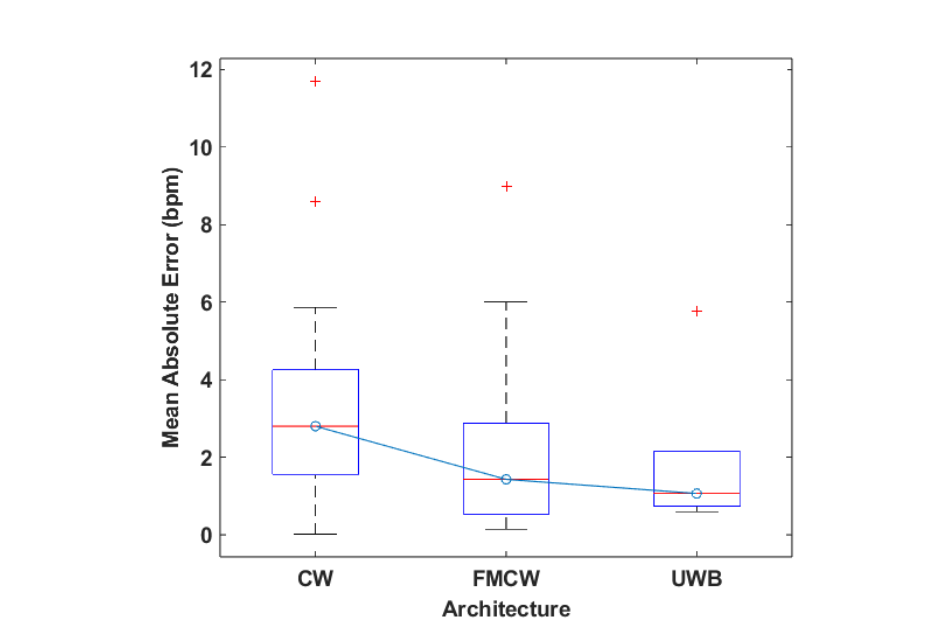
\includegraphics[width=0.7\linewidth]{Images/chapter3/3-2.png}
    \caption{ نمودار جعبه‌ای مقادیر \lr{MAE} برای هر معماری.\cite{frazao2024radar}.}
    \label{fig:fmcw_vitals}
\end{figure}

\subsection{عملکرد آزمایشگاهی و خطاهای اندازه‌گیری}
\label{sec:experimental-performance}

بررسی داده‌های منتشرشده در ۵۶ مطالعه‌ی اندازه‌گیری ضربان قلب نشان می‌دهد که معماری \lr{FMCW} کمترین میانه‌ی خطای مطلق (\lr{MAE}) را دارد، در حالی که \lr{CW} بیشترین میانه‌ی خطا را به خود اختصاص داده است. اگرچه \lr{UWB} در مقایسه‌ی تعداد مطالعات کمتر است، دامنه خطای این معماری کوچک‌تر بوده اما برای تأیید برتری آن نیاز به مطالعات بیشتر است.

به‌طور خاص، در شکل جعبه‌ای (\lr{Boxplot}) مقایسه خطاها، معماری \lr{CW} دارای بالاترین میانه و دامنه‌ی گسترده‌تری از خطا است، در حالی که \lr{FMCW} توزیع خطا فشرده‌تر و \lr{UWB} پایین‌ترین مقادیر حداکثر خطا را نشان می‌دهد. این نتایج گویای برتری معماری \lr{FMCW} در سنجش غیرتماسی ضربان قلب به‌واسطه‌ی مقاومت آن در برابر نویز و تداخل محیطی است.

% \subsection{نتیجه‌گیری موقت}
% \label{sec:interim-conclusion}

% با توجه به مقایسه‌ی مزایا، معایب و داده‌های تجربی، معماری \lr{FMCW} گزینه‌ی اول برای سامانه‌های پزشکی غیرتماسی محسوب می‌شود. \lr{CW} علیرغم سادگی، به‌دلیل عدم امکان تفکیک فاصله و حساسیت بالا به نویز به‌عنوان جایگزین دوم مطرح است و \lr{UWB}، هرچند پتانسیل دقت بالایی دارد، به‌علت پیچیدگی سخت‌افزاری و کمبود مطالعات بالینی گسترده، هنوز در مرحله آزمایشگاهی قرار دارد. در فصل‌های بعدی، بسته به نیازمندی‌های بالینی و محدودیت‌های سخت‌افزاری، انتخاب معماری مناسب برای طراحی سامانه‌ی پایان‌نامه تشریح خواهد شد.
